\subsubsection{Interrupts and Interrupt Handler}

The \textbf{interrupts change the normal flow of control}. As you can see in Figure \ref{fig: Program and Interrupt Handler}, on the left we see the instructions of the program; on the right we see the interrupt handler.

\begin{figure}[!htp]
    \centering
    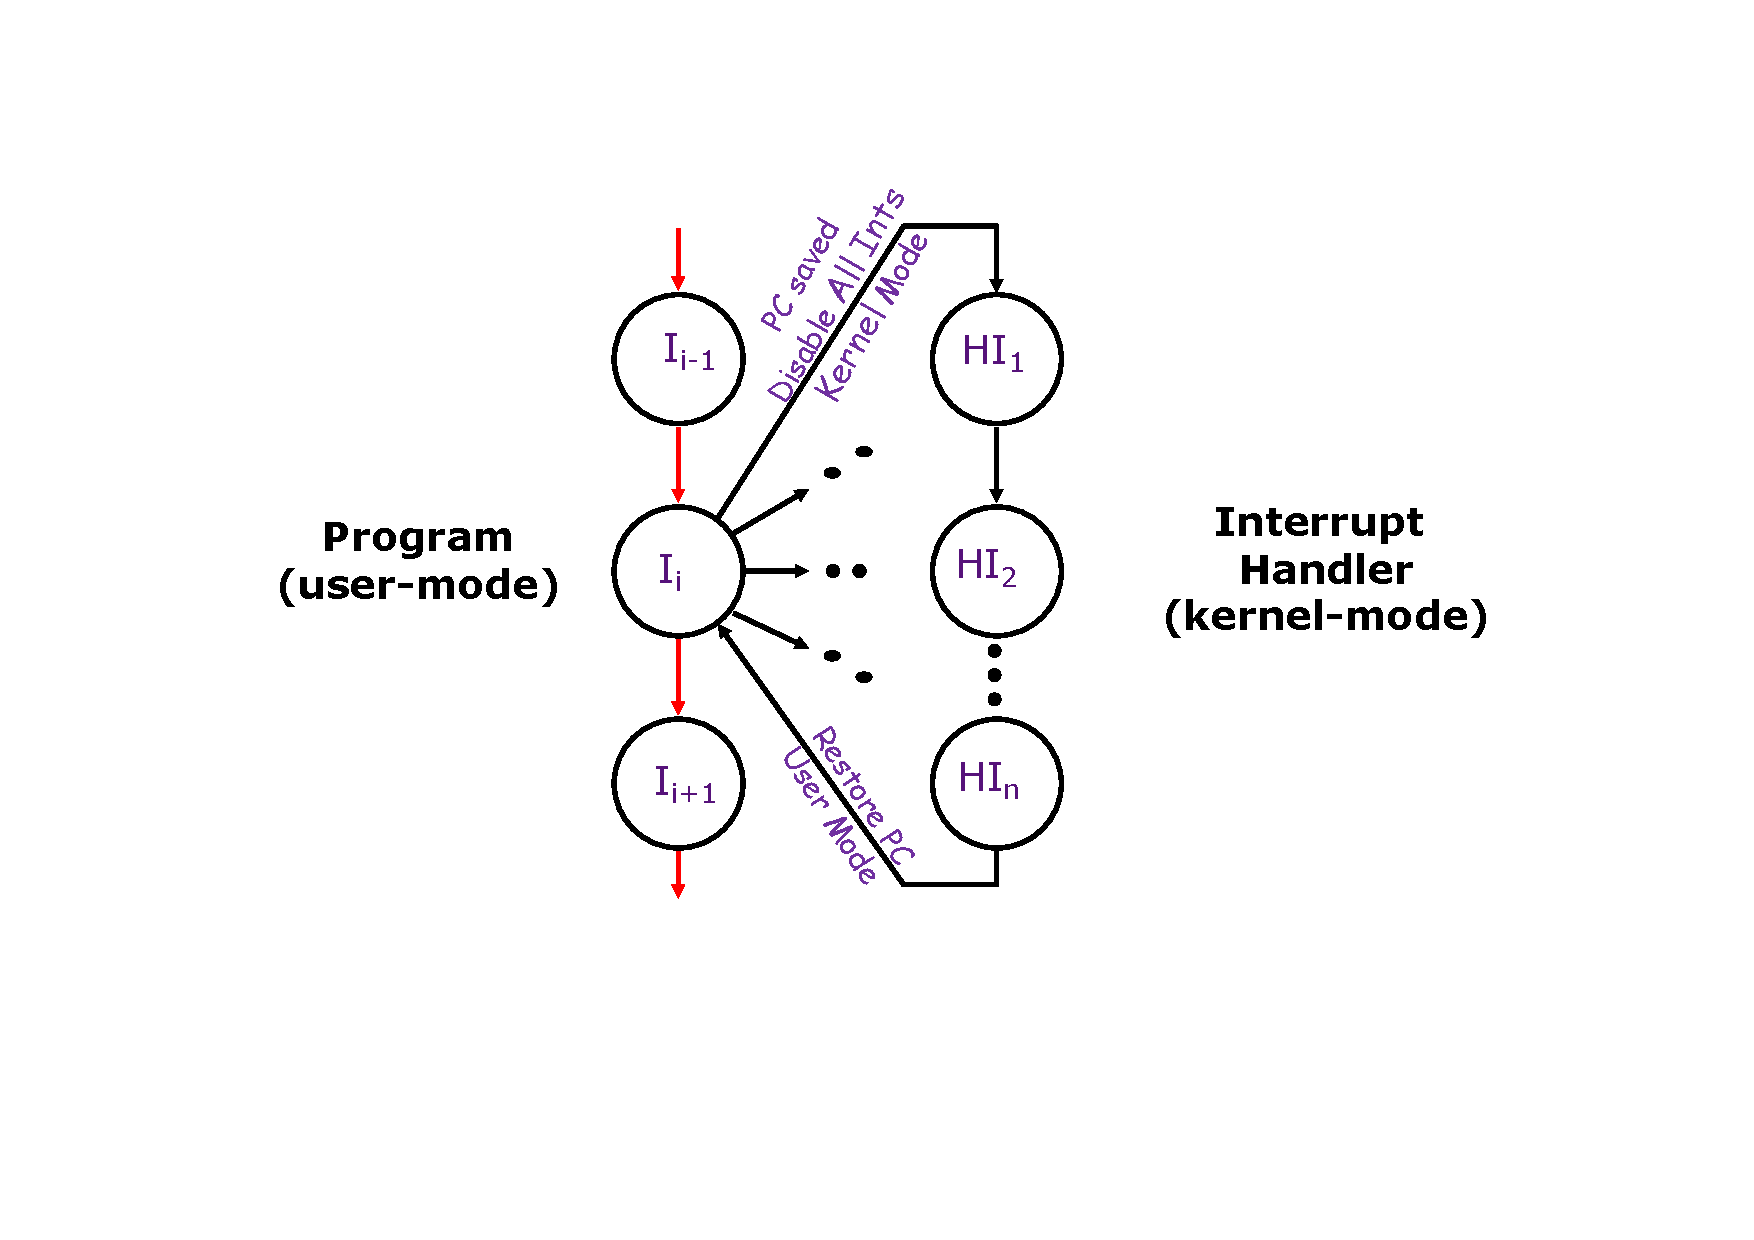
\includegraphics[width=.8\textwidth]{img/interrupts-1.pdf}
    \caption{Program and Interrupt Handler.}
    \label{fig: Program and Interrupt Handler}
\end{figure}

\noindent
An \indexdefinition{Interrupt Handler}, also known as an \textbf{interrupt service routine} or \textbf{ISR}, is a special \textbf{block of code associated with a specific interrupt condition}. Interrupts can be of two types:
\begin{itemize}
    \item \indexdefinition{Synchronous Interrupts} (exception) are caused by a particular instruction stage. In general, the \textbf{instruction} $I_{i}$ (see the Figure \ref{fig: Program and Interrupt Handler}) \textbf{cannot be completed} and needs to be \textbf{restarted after the exception has been handled}.
    
    If we think about the pipeline, this condition requires undoing the effect of one or more partially executed instructions.


    \item \indexdefinition{Asynchronous Interrupts} are caused by an I/O device requesting attention by asserting one of the prioritized interrupt request lines.
    
    When the processor decides to process the interrupt:
    \begin{enumerate}
        \item It stops the current program at instruction $I_{i}$, completing all the instructions up to $I_{i-1}$ (called \textbf{precise interrupt}, see below to understand what it is).
        
        \item It saves the Program Counter (PC) of the instruction $I_{i}$ in a special register called \indexdefinition{Exception Program Counter (EPC)}: $\texttt{PC} \rightarrow \texttt{EPC}$.
        
        \item It disables interrupts and transfer control to a designated interrupt handler running in the \textbf{kernel mode}. So it loads the \indexdefinition{Interrupt Vector Address (IVA)} into the Program Counter (PC): $\texttt{IVA} \rightarrow \texttt{PC}$.
        
        \newpage

        \item When the Interrupt Handler has finished, it must \textbf{restore the stable situation}. It uses a \textbf{special indirect jump instruction} called \indexdefinition{Return-From-Exception (RFE)}, which restores the PC and:
        \begin{itemize}
            \item Re-enables the interrupts (again, because they were disabled in the previous step);
            
            \item Returns the processor to user mode;
            
            \item Restores the hardware and control state.
        \end{itemize}
    \end{enumerate}
\end{itemize}

\begin{flushleft}
    \textcolor{Green4}{\faIcon{question-circle} \textbf{Ok, but what exactly is a Precise Interrupts in Asynchronous Interrupts?}}
\end{flushleft} \index{Precise Interrupts}\index{Precise Exceptions}
An \textbf{interrupt} or \textbf{exception} is \textbf{precise} if there is a single instruction (or interrupt point) for which all \textbf{previous instructions} have \textbf{committed their state} and \textbf{no subsequent instructions} (including the interrupting instruction $I_{i}$) have \textbf{changed any state}.

\highspace
In other words, we can restart execution at the interrupt point and \dquotes{get the right answer}.

\begin{figure}[!htp]
    \centering
    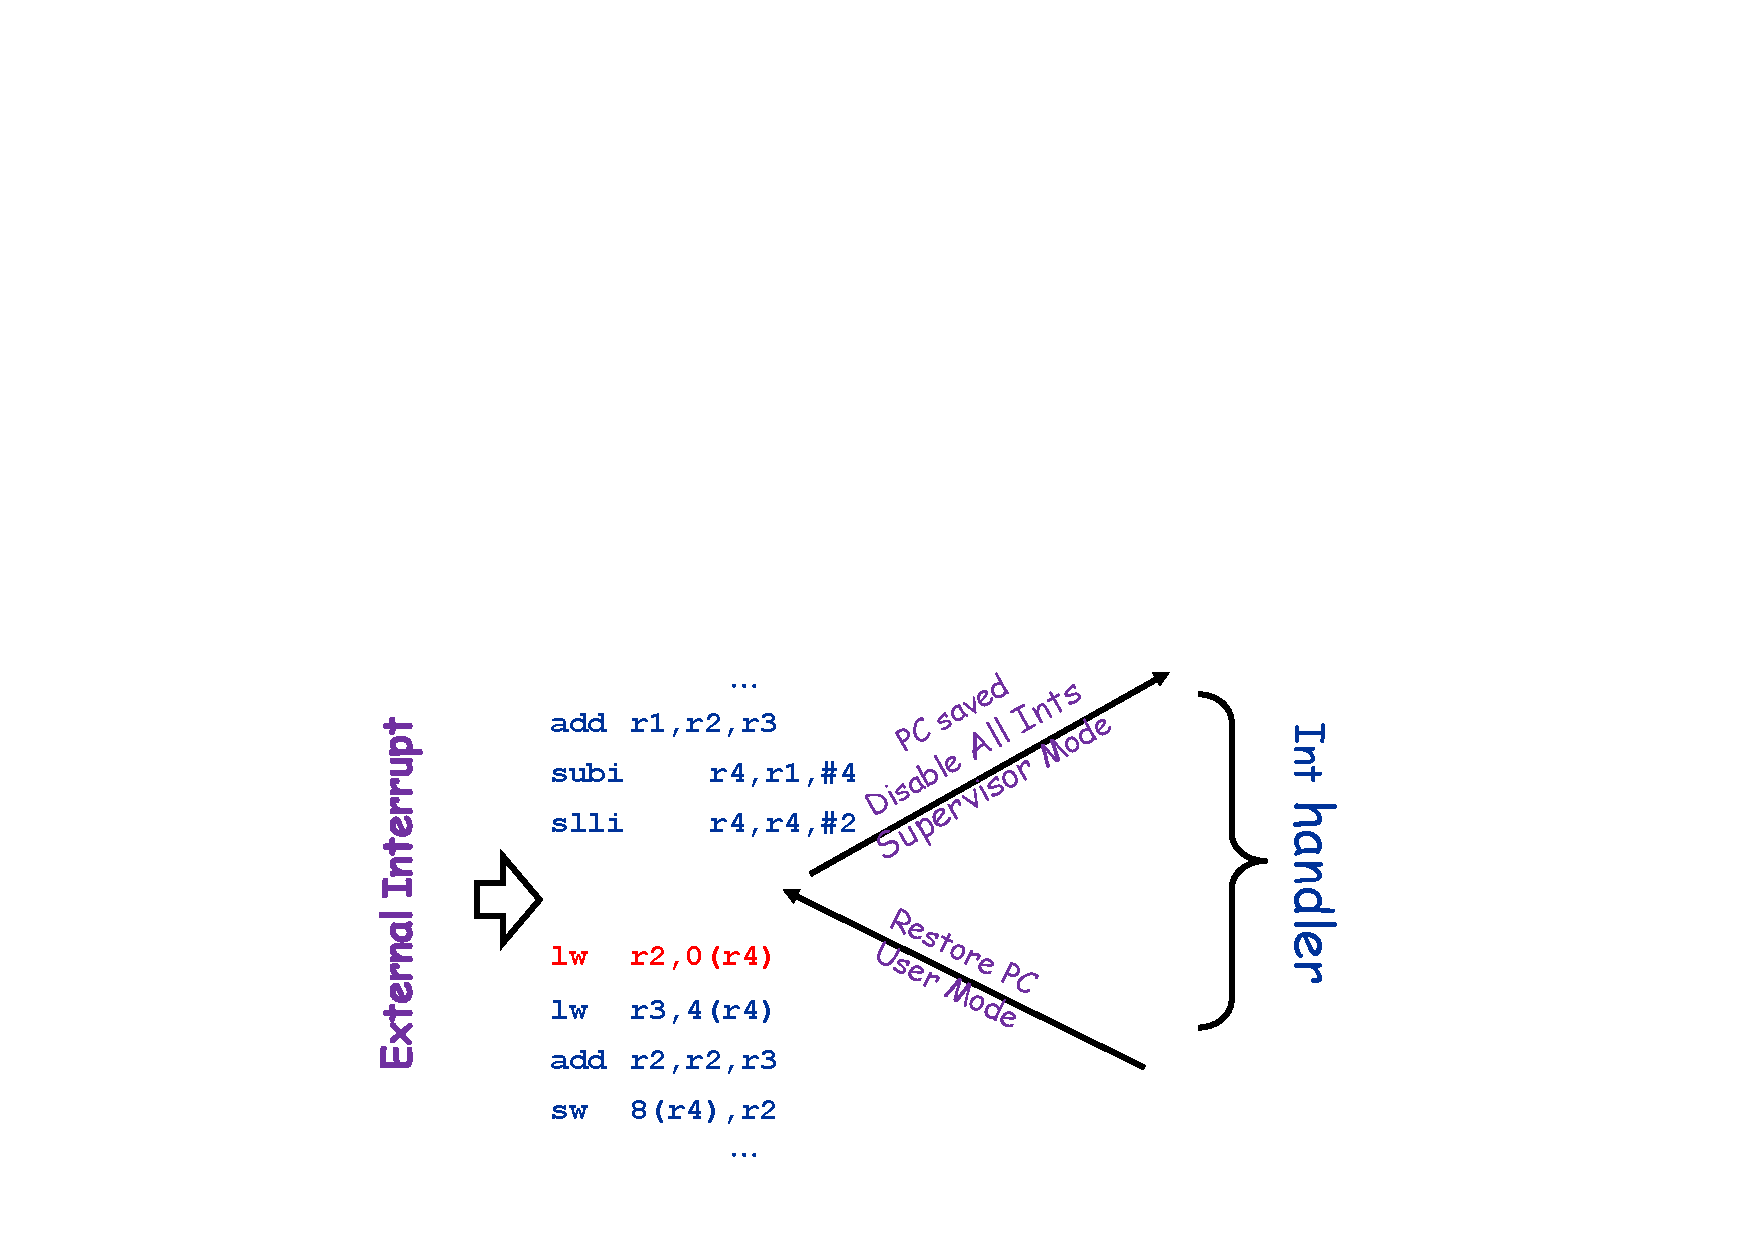
\includegraphics[width=.8\textwidth]{img/precise-interrupts-1.pdf}
    \caption{\example{Example} of precise interrupt/exception.}
\end{figure}